\documentclass[a4paper]{article}

\usepackage{fontspec}
\usepackage{mathpazo}
\setmainfont
     [ BoldFont       = texgyrepagella-bold.otf ,
       ItalicFont     = texgyrepagella-italic.otf ,
       BoldItalicFont = texgyrepagella-bolditalic.otf ]
     {texgyrepagella-regular.otf}
\setmainfont{Gill Sans MT}

\usepackage[english]{babel}
\usepackage[utf8]{inputenc}
\usepackage{amsmath}
\usepackage{graphicx}
\usepackage[colorinlistoftodos]{todonotes}
\usepackage{physics}

%\DeclareMathOperator{\Tr}{Tr}

\title{Convex Optimization - Homework 6: Applications}

\author{David McPherson}

\date{\today}

\begin{document}
\maketitle

\section{Exercise 1: Two Stage Decision Making}
\subsection{Demand Measured prior to Purchase}

The linear program formulation for maximizing profit is:

\begin{equation}
\max \left \{ [\begin{matrix}25 & 10\end{matrix}]\left [\begin{matrix}s_1 \\ s_2 \end{matrix} \right ]
-[\begin{matrix}3.50 & 2.60 & -6.80\end{matrix}] \left [\begin{matrix}x_1 \\ x_2 \\ x_3 \end{matrix} \right ]
\right \}
\end{equation}

subject to

\begin{equation}
s_i \leq D_i , \forall i \in \{1,2\}
\end{equation}
\begin{equation}
s_i \leq y_i , \forall i \in \{1,2\}
\end{equation}
\begin{equation}
\left[
\begin{matrix}
3 & 1 \\
1 & 0 \\
1 & 1 \\
\end{matrix}
\right]
\left[\begin{matrix}y_1 \\ y_2\end{matrix}\right]
\leq
\left[\begin{matrix}x_1 \\ x_2 \\ x_3 \end{matrix}\right]
\end{equation}

where $y_i$ is the quantity of drug $i$ produced, $s_i$ is the quantity of drug $i$ sold, $D_i$ is the quantity of drug $i$ demanded, and $x_i$ is the quantity of ingredient $i$ purchased.

Implementing this formulation in CVX with a demand of $D_1 = 150$ and $D_2 = 200$ yields a profit of \$765 by producing and selling 150 units of Drug 1 and 0 units of Drug 2. To produce this, 450 units of Ingredient 1, 150 units of Ingredient 2, and 150 units of Ingredient 3 were acquired.

\subsection{Profit Maximization for Three Demand Scenarios}
The same formulation (with knowing the demand ahead of purchasing, producing, and selling) was used to maximize profit for each of the three demand scenarios. The maximum profit and associated drug production, selling, and ingredient purchases are filed in Table 1.

\begin{tabular}{c  c  c c  c c c c c}
           & Profit & $s_1$ & $s_2$ & $y_1$ & $y_2$ & $x_1$ & $x_2$ & $x_3$ \\
Scenario 1 &  510   & 100   & 0     & 100   & 0     & 300   & 100   & 100   \\
Scenario 2 &  765   & 150   & 0     & 150   & 0     & 450   & 150   & 150   \\
Scenario 3 & 1020   & 200   & 0     & 200   & 0     & 600   & 200   & 200   \\
\end{tabular}

Note that no amount of Drug 2 was produced, since we produce a \$0.60 loss with each sale.

\subsection{Demand Measured prior to Selling}
Both of the above analyses assume perfect information with demand being known before ingredients are acquired and any manufacturing takes place.
However, a more realistic scenario would be one where we only learn demand after acquisition and assembly has already taken place.
Now we need to optimize one choice of the $x_i$ and $y_1$ such that the expected profit is maximized.
We will use superscripts to denote versions of the variables that depend on the scenario.
In this analysis, we have $s_i^j$ denoting the amount of drug $i$ sold in demand scenario $j$ and $D_i^j$ denoting the demand for drug $i$ in the same scenario $j$.
Therefore our expected profit optimization problem can be formulated as:

\begin{equation}
\max \left \{ [\begin{matrix}25 & 10\end{matrix}]
\left( 0.2 \left [\begin{matrix}s_1^1 \\ s_2^1 \end{matrix} \right ] + 0.5 \left [\begin{matrix}s_1^2 \\ s_2^2 \end{matrix} \right ] + 0.3 \left [\begin{matrix}s_1^3 \\ s_2^3 \end{matrix} \right ] \right)
-[\begin{matrix}3.50 & 2.60 & -6.80\end{matrix}] \left [\begin{matrix}x_1 \\ x_2 \\ x_3 \end{matrix} \right ]
\right \}
\end{equation}

subject to

\begin{equation}
s_i^j \leq D_i^j , \forall i \in \{1,2\} , \forall j \in \{1,2,3\}
\end{equation}
\begin{equation}
s_i^j \leq y_i , \forall i \in \{1,2\} , \forall j \in \{1,2,3\}
\end{equation}
\begin{equation}
\left[
\begin{matrix}
3 & 1 \\
1 & 0 \\
1 & 1 \\
\end{matrix}
\right]
\left[\begin{matrix}y_1 \\ y_2\end{matrix}\right]
\leq
\left[\begin{matrix}x_1 \\ x_2 \\ x_3 \end{matrix}\right]
\end{equation}

Solving this formulation in CVX results in an expected profit of \$515.00 with

\begin{tabular}{c  c  c c  c c c c c}
           & Profit & $s_1$ & $s_2$ & $y_1$ & $y_2$ & $x_1$ & $x_2$ & $x_3$ \\
Scenario 1 & -485   & 100   & 0     &       &       &       &       &       \\
Scenario 2 &  765   & 150   & 0     & 150   & 0     & 450   & 150   & 150   \\
Scenario 3 &  765   & 150   & 0     &       &       &       &       &       \\
\end{tabular}

\subsection{Demand Measured prior to Manufacture}
A slightly better scenario would be if information on the drug demand was received prior to manufacture but after ingredient acquisition.
In this case, we need to optimize one choice of the $x_i$ such that the expected profit is maximized (we can tailor the $y_i$ and $s_i$ to the demand scenario).
Now, our expected profit optimization problem can be formulated as:

\begin{equation}
\max \left \{ [\begin{matrix}25 & 10\end{matrix}]
\left( 0.2 \left [\begin{matrix}s_1^1 \\ s_2^1 \end{matrix} \right ] + 0.5 \left [\begin{matrix}s_1^2 \\ s_2^2 \end{matrix} \right ] + 0.3 \left [\begin{matrix}s_1^3 \\ s_2^3 \end{matrix} \right ] \right)
-[\begin{matrix}3.50 & 2.60 & -6.80\end{matrix}] \left [\begin{matrix}x_1 \\ x_2 \\ x_3 \end{matrix} \right ]
\right \}
\end{equation}

subject to

\begin{equation}
s_i^j \leq D_i^j , \forall i \in \{1,2\} , \forall j \in \{1,2,3\}
\end{equation}
\begin{equation}
s_i^j \leq y_i^j, \forall i \in \{1,2\} , \forall j \in \{1,2,3\}
\end{equation}
\begin{equation}
\left[
\begin{matrix}
3 & 1 \\
1 & 0 \\
1 & 1 \\
\end{matrix}
\right]
\left[\begin{matrix}y_1^j \\ y_2^j\end{matrix}\right]
\leq
\left[\begin{matrix}x_1 \\ x_2 \\ x_3 \end{matrix}\right]
, \forall j \in \{1,2,3\}
\end{equation}

Solving this formulation in CVX results in an expected profit of \$615.00 with

\begin{tabular}{c  c  c c  c c c c c}
           & Profit & $s_1$ & $s_2$ & $y_1$ & $y_2$ & $x_1$ & $x_2$ & $x_3$ \\
Scenario 1 &   15   & 100   & 50    & 100   & 50    &       &       &       \\
Scenario 2 &  765   & 150   & 0     & 150   & 0     & 450   & 150   & 150   \\
Scenario 3 &  765   & 150   & 0     & 150   & 0     &       &       &       \\
\end{tabular}

\section{Exercise 2: Dicsount Factor Curve Fitting }
\subsection{Formulation}
The formulation for this problem is:

\begin{equation}
\begin{aligned}
\min_a & \sum_{i=1}^I | p_0 f(t_0^{(i)}) +  p_1 f(t_1^{(i)}) |
\\ = \min_a & \sum_{i=1}^I | p_0 (a_{0,k_{i0}} + a_{1,k_{i0}} t_0^{(i)} + a_{2,k_{i0}} t_0^{(i) 2} )
+  p_1 (a_{0,k_{i1}} + a_{1,k_{i1}} t_1^{(i)} + a_{2,k_{i1}} t_1^{(i) 2} ) |
\end{aligned}
\end{equation}

where $k_{ij}$ is the interval that $t_j^{(i)}$ falls in.

Subject to the constraints:

\begin{equation}
  \begin{aligned}
    a_{0,k} + a_{1,k} m_{k+1} + a_{2,k} m_{k+1}^2
    &=
    a_{0,k+1} + a_{1,k+1} m_{k+1} + a_{2,k+1} m_{k+1}^2
    , &\forall k \in \{1,2,\dots,N-1\}
    \\
    a_{1,k} + 2 a_{2,k} m_{k+1}
    &=
    a_{1,k+1} + 2 a_{2,k+1} m_{k+1}
    , &\forall k \in \{1,2,\dots,N-1\}
    \\
    a_{1,k} + 2 a_{2,k} m_k     &\leq 0 , & \forall k \in \{1,2,\dots,N\}
    \\
    a_{1,k} + 2 a_{2,k} m_{k+1} &\leq 0 , & \forall k \in \{1,2,\dots,N\}
    \\
    a_{0,N} + a_{1,N} T + a_{2,N} T^2 &\geq 0 &
  \end{aligned}
\end{equation}

\subsection{CVX Solution}
A MATLAB script was written up to solve this formulation using CVX.
The resultant discount curve fits are shown in Figs. 1-4 below, with their error values in the caption.

\begin{figure}[!ht]
  \centering
  \begin{minipage}[b]{0.4\textwidth}
    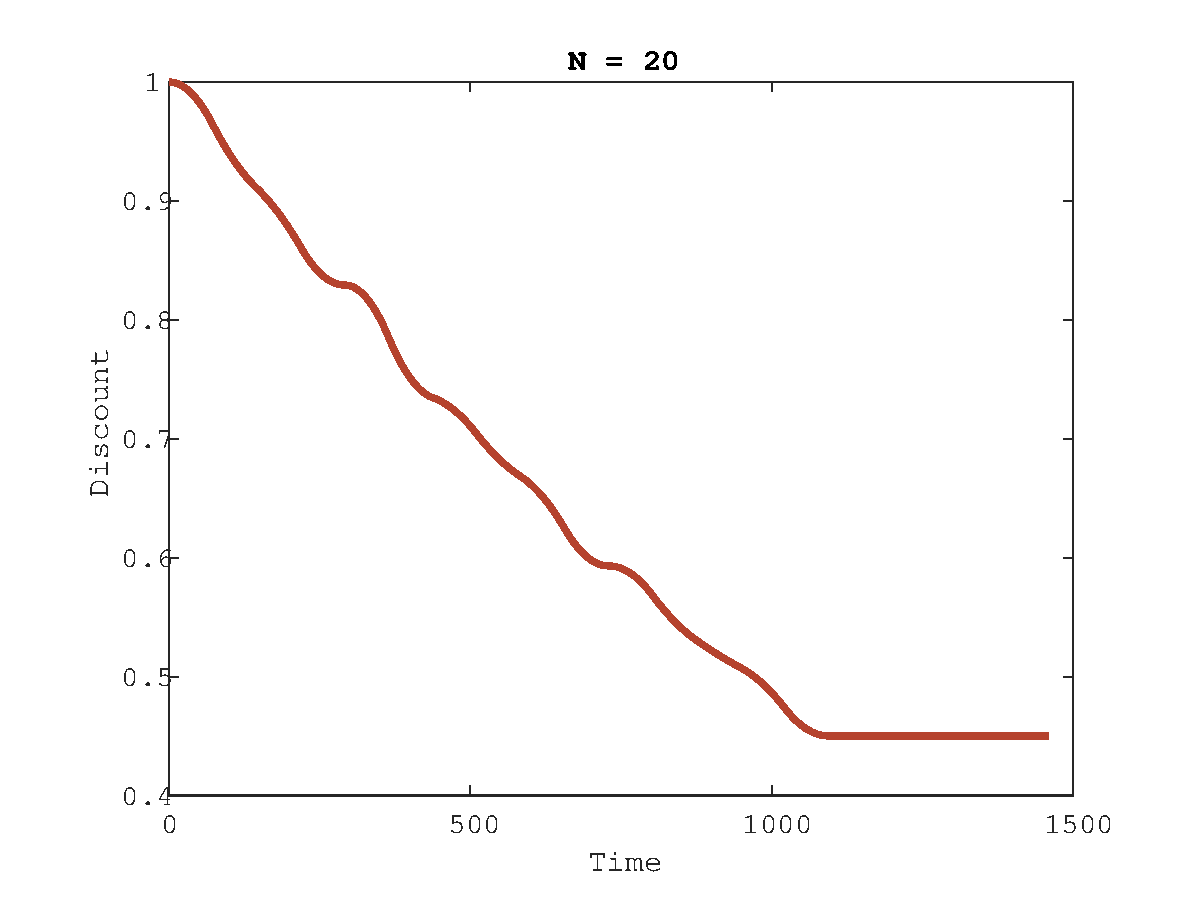
\includegraphics[width=1.0\textwidth]{N20.eps}
    \caption{Discount Curve fit for N=20 (optimum error = 1.53704)}
  \end{minipage}
  \hfill
  \begin{minipage}[b]{0.4\textwidth}
    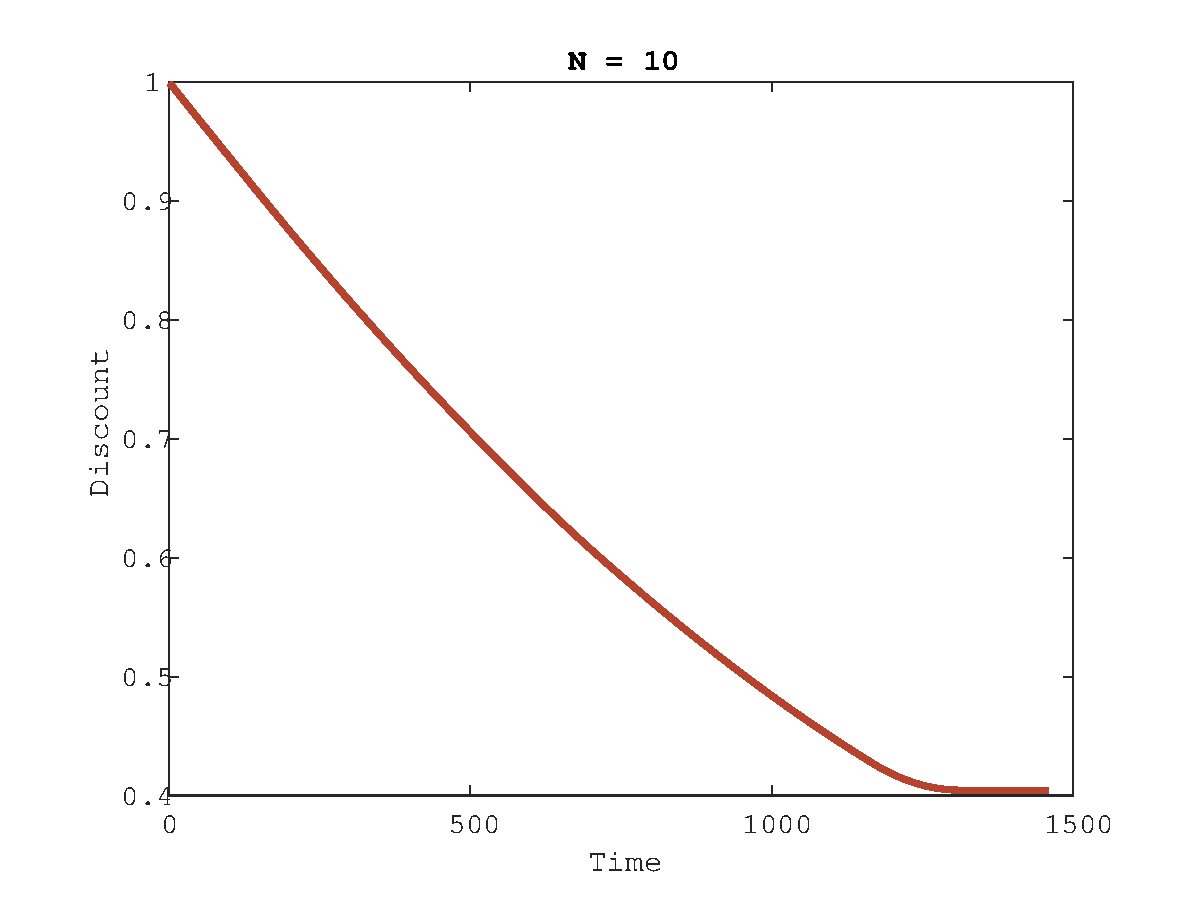
\includegraphics[width=1.0\textwidth]{N10.eps}
    \caption{Discount Curve fit for N=10 (optimum error = 1.73544)}
  \end{minipage}
\end{figure}

\begin{figure}[!ht]
  \centering
  \begin{minipage}[b]{0.4\textwidth}
    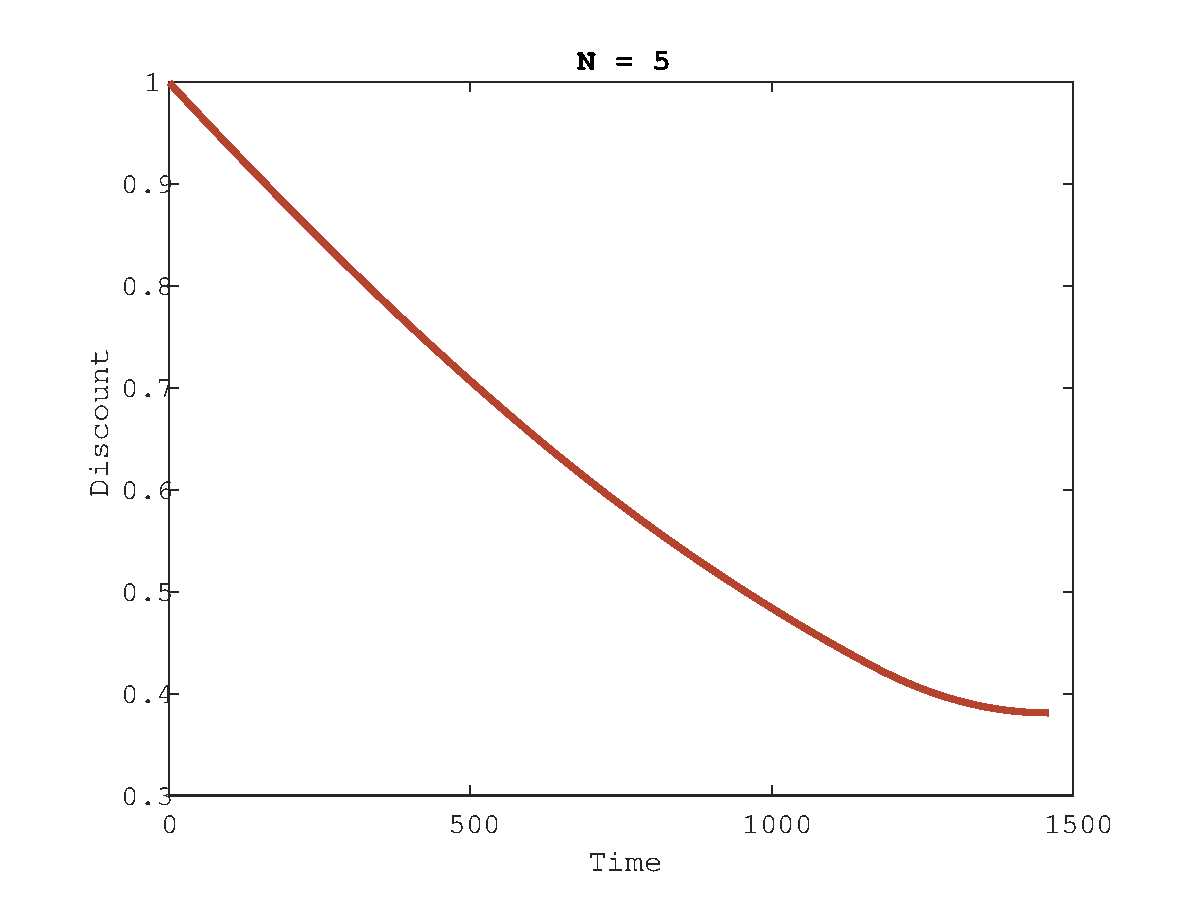
\includegraphics[width=1.0\textwidth]{N5.eps}
    \caption{Discount Curve fit for N=5 (optimum error = 2.0067)}
  \end{minipage}
  \hfill
  \begin{minipage}[b]{0.4\textwidth}
    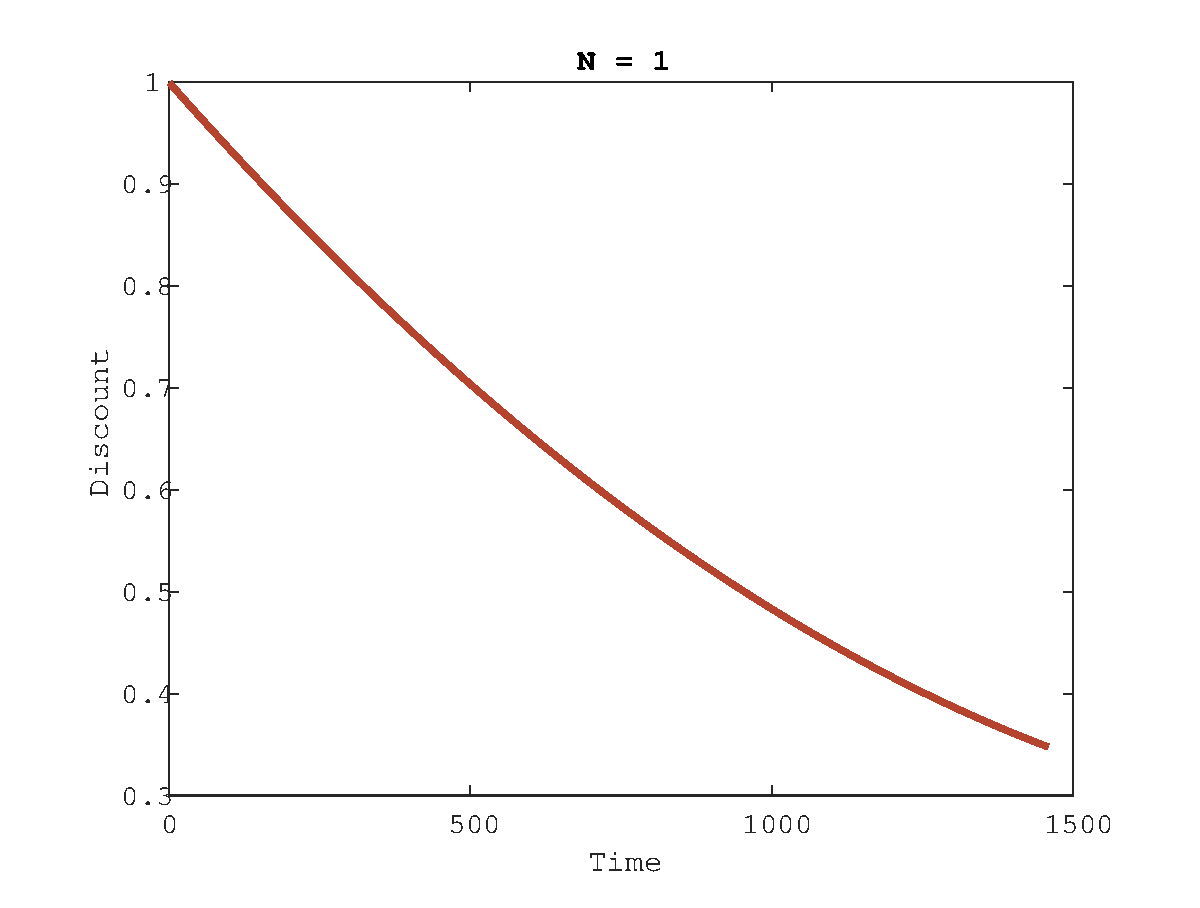
\includegraphics[width=1.0\textwidth]{N1.eps}
    \caption{Discount Curve fit for N=1 (optimum error = NaN)}
  \end{minipage}
\end{figure}

\section{Exercise 3: Probability Density Estimation}
\subsection{Reward Function}
Let $F$ be the true distribution from which the ten samples $x_i$ are drawn.
The optimization problem which gives the maximum likelihood estimator $f$ is:

\begin{equation*}
\begin{aligned}
& \underset{f}{\text{maximize}}
&  \Pi_{i=1}^{10} f(x) \\
& \text{subject to}
&  \int_X f(x) dx = 1 \\
& & f(x) \geq 0, \; \forall x
\end{aligned}
\end{equation*}

Since the $\log$ function is monotone increasing, this is an equivalent optimization problem to:

\begin{equation*}
\begin{aligned}
& \underset{f}{\text{maximize}}
&  \log \left( \Pi_{i=1}^{10} f(x) \right) \\
& &  = \sum_{i=1}^{10} \log(f(x)) \\
& \text{subject to}
&  \int_X f(x) dx = 1 \\
& & f(x) \geq 0, \; \forall x
\end{aligned}
\end{equation*}

"Equivalent" in the sense that the optimization problem has the same minimizing choice of $f^*(x)$,
if not necessarily the same optimal value $p^*$.

\subsection{Optimization Formulation}
Define the interval that $x_i$ falls on to be from 0 to $X$.
To divide this interval into $N$ evenly spaced sub-intervals, each sub-interval must be $r=X/N$.
Therefore the formulation is:

\begin{equation*}
\begin{aligned}
& \underset{c,d}{\text{maximize}}
& \sum_{i=1}^{10} \log(c_{i_j}(x - i_j r - r) + d_{i_j}) &\\
& \text{subject to}
&  \sum_{i=1}^{N} (d_i r + \frac{1}{2} c_i r^2) = 1 & \\
& & d_i \geq 0,               & & \forall i \in {1,\dots,N} \\
& & d_i + c_i r \geq 0,       & & \forall i \in {1,\dots,N} \\
& & d_{i+1} = d_i + c_i r,    & & \forall i \in {1,\dots,N-1} \\
\end{aligned}
\end{equation*}

Note here that we define our parameters $c_i$ and $d_i$ as a line with respect to interval-local coordinates rather than global coordinates.
The interval-local coordinates start at 0 and range up to $r$ when the interval ends.
To transform from the universal coordinates $x$ into the local coordinates use $x' = c_{i_j}(x - i_j r - r) $ like we do in the objective function.
This definition in local coordinates greatly simplifies the definition of the constraints as the borders are always at 0 and $r$.

\subsection{CVX Solution}
A Matlab script for optimizing this formulation using CVX was composed and ran.
The resulting best fit corresponded approximately to a sum of Kroniker deltas at each sample point each weighted to make the total sum to 1 (as constrained, since this is a PDF).
The plot is shown in Fig. 5 along with the baseline and some future fits to be described in the following sections.
Note that the plot is clipped since and that these "deltas"  actually stretch extremely high up to around 25.
This clipping is to keep the other fits and the baseline visible.

\begin{figure}[ht!]
\centering
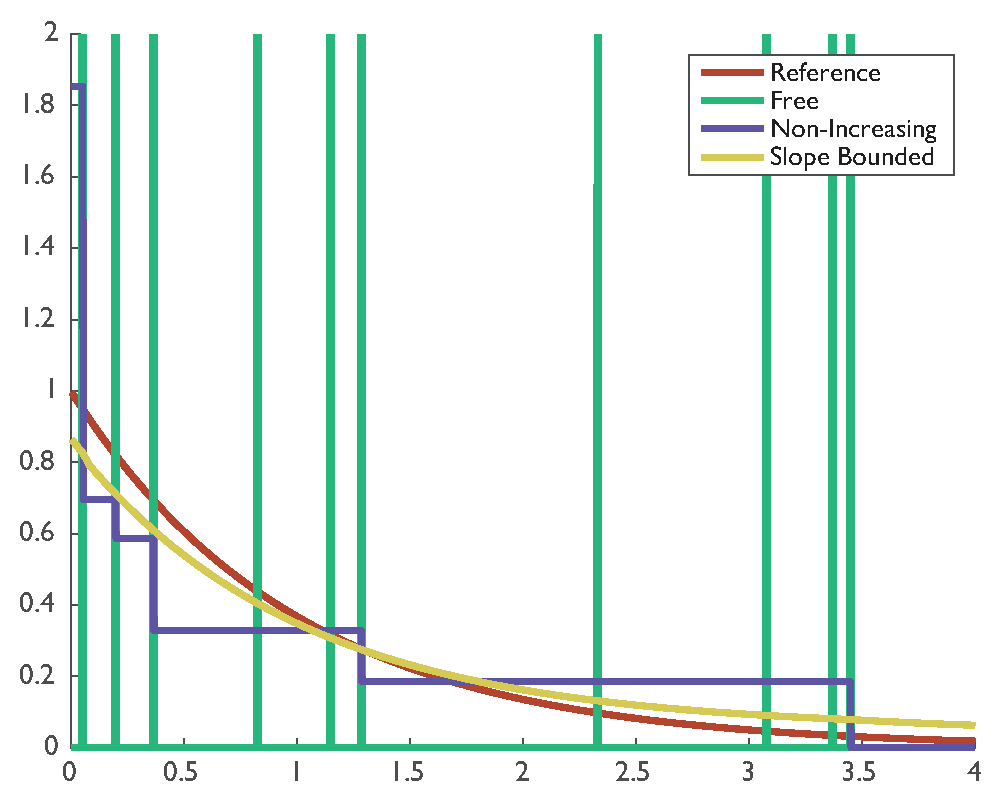
\includegraphics[width=0.9\textwidth]{Question3f.eps}
\caption{Probability Density Function Fits}
\end{figure}

\subsection{Non-Increasing Requirement}
We want to encode that the PDF is non-decreasing.
That is to that higher values of $x$ were never more likely than lower values.
This requirement becomes one additional constraint.
Our elegant interval-local coordinate parametrization simplifies this constraint to just:

\begin{equation}
  c_i \leq 0 \; \forall i
\end{equation}

Adding this constraint to our CVX optimization results in the plot labeled "Non-Increasing" in Fig. 5.
Note how much better this PDF estimation is then the drastically over-fit "deltas" from the previous optimization.

\subsection{Bounded Slope Requirements}
Since our true PDF is an exponential with mean 1, the true slope of this PDF is:

$$
\frac{df}{dx} = -e^{-x}
$$

To encode $\pm 20\%$ bounds on the slope at all times we use:

\begin{equation}
  \begin{aligned}
    c_i \leq -0.8 e^{-x} & \forall x \in I_i \rightarrow & c_i \leq -0.8 e^{-r(i-1)} \\
    c_i \geq -1.2 e^{-x} & \forall x \in I_i \rightarrow & c_i \geq -1.2 e^{-ri}
  \end{aligned}
\end{equation}

where the implication step was made by choosing the tightest bound in the interval $I_i$.

Adding this constraint produces the closest approximation to the true PDF as plotted in Fig. 5.

\end{document}
